%%%%%%%%%%%%%%%%%%%%%%%%%%%%%%%%%%%%%%%%%%%%%%
%                insertmeeting
% 1) Title (something creative & funny?)
% 2) Date (MM/DD/YYYY)
% 3) Location (ex. Hagerty High School)
% 4) People/Committees Present 
% 5) Picture 
% 6) Start Time & Stop Time (ex. 12:30AM to 4:30PM)
%%%%%%%%%%%%%%%%%%%%%%%%%%%%%%%%%%%%%%%%%%%%%%
\insertmeeting 
	{Christmas Season} 
	{12/01/21}
	{Hagerty High School}
	{Anouska, James, Ritam}
	{Images/RobotPics/robot.jpg}
	{2:30 - 4:30}
	
\hhscommittee{Software}
\noindent\hfil\rule{\textwidth}{.4pt}\hfil
\subsubsection*{Goals}
\begin{itemize}
    \item Start on opencv hough circle transform   

\end{itemize} 

\noindent\hfil\rule{\textwidth}{.4pt}\hfil

\subsubsection*{Accomplishments}
Today, we started by researching hough circle detection as a back up vision program. We looked at OpenCV documentation about the hough circle transform. We found premade code and one of our mentors, Mr. Harper, helped us by putting it into the Eclipse IDE. This allowed multiple people to work on the robot without needing to physically use it. We also glued some circles on top of each other on a piece of paper so we could test the vision with it. We used sliders in Eclipse that allowed us to test different values for the minimum and maximum radius. When testing the vision, it found our circles as well as others in the background by drawing outlines on them. We tested it with a picture of a compass and it was able to draw one outline, so we knew we had to make it more specific. We then saw we needed to change the distance between the centers. They were on top of each other so there was no distance between them. Since the circles' centers could not be overlapping, we planned on printing new circles where their centers would be separate. This would allow us to find the distance between the two circles that have the same radius.

\hhscommittee{Hardware}
\noindent\hfil\rule{\textwidth}{.4pt}\hfil
\subsubsection*{Goals}
\begin{itemize}
    \item Build and test roller intake
	\item Resolve any issues that arise with new design and create a final version


\end{itemize} 

\noindent\hfil\rule{\textwidth}{.4pt}\hfil

\subsubsection*{Accomplishments}
With all of the 3d printed parts hot off the printer, we came into today’s meeting ready to give our roller intake its first test. Printed out of PLA on a member’s personal 3D printer, this intake was meant to be a prototype to see both how  the concept functions and if any of the parts of the design need to be changed before printing with more expensive, but higher quality printers at UCF. To prepare for our test, we started by creating what would actually be used for the roller, a piece of surgical tubing attached to a shaft. Next pressed bearings into the holes of the 3d printed parts to make the roller roll smoother.Using some REV hex shafts, we fitted the roller and newly printed larger o-belt pulleys onto the intake. Now we were finally ready to test. Because we don’t yet want to buy belts for the current intake design which is subject to change, we hooked the shaft up to a drill and tried to see how well it sucked in blocks. As we were testing, we found that although the intake sometimes had a hard time gripping the blocks before fully coming in contact with the roller, it was able to pick up blocks quite a bit faster than our old clamp mechanism. Before we could take any pictures, however, the intake started to crack and soon after completely broke at a weak point surrounding a bearing (Figure \ref{fig:120121-1}). This influenced us to change the design to make the plastic a bit thicker around the arm where it broke. We also plan on printing at UCF next time to use better filament like nylon that won't break nearly as easily. Although we came up with this plan, much of it will have to wait to be implemented. Because we wnat to allow time for driver practice and autonoumous in addition to semester exams taking place at our school in the next 2 weeks, we are most liekely going to stick with our original grabber intake for now. this way, we wont end up with an unreliable and potentially nonfunctioning intake if we run out of time completely in the next 2 weeks. We still plan on using the roller intake in the future though. Instead, we plan to fix and use our old intake and want to work on some cad for more future plans.

\begin{figure}[htp]
\centering
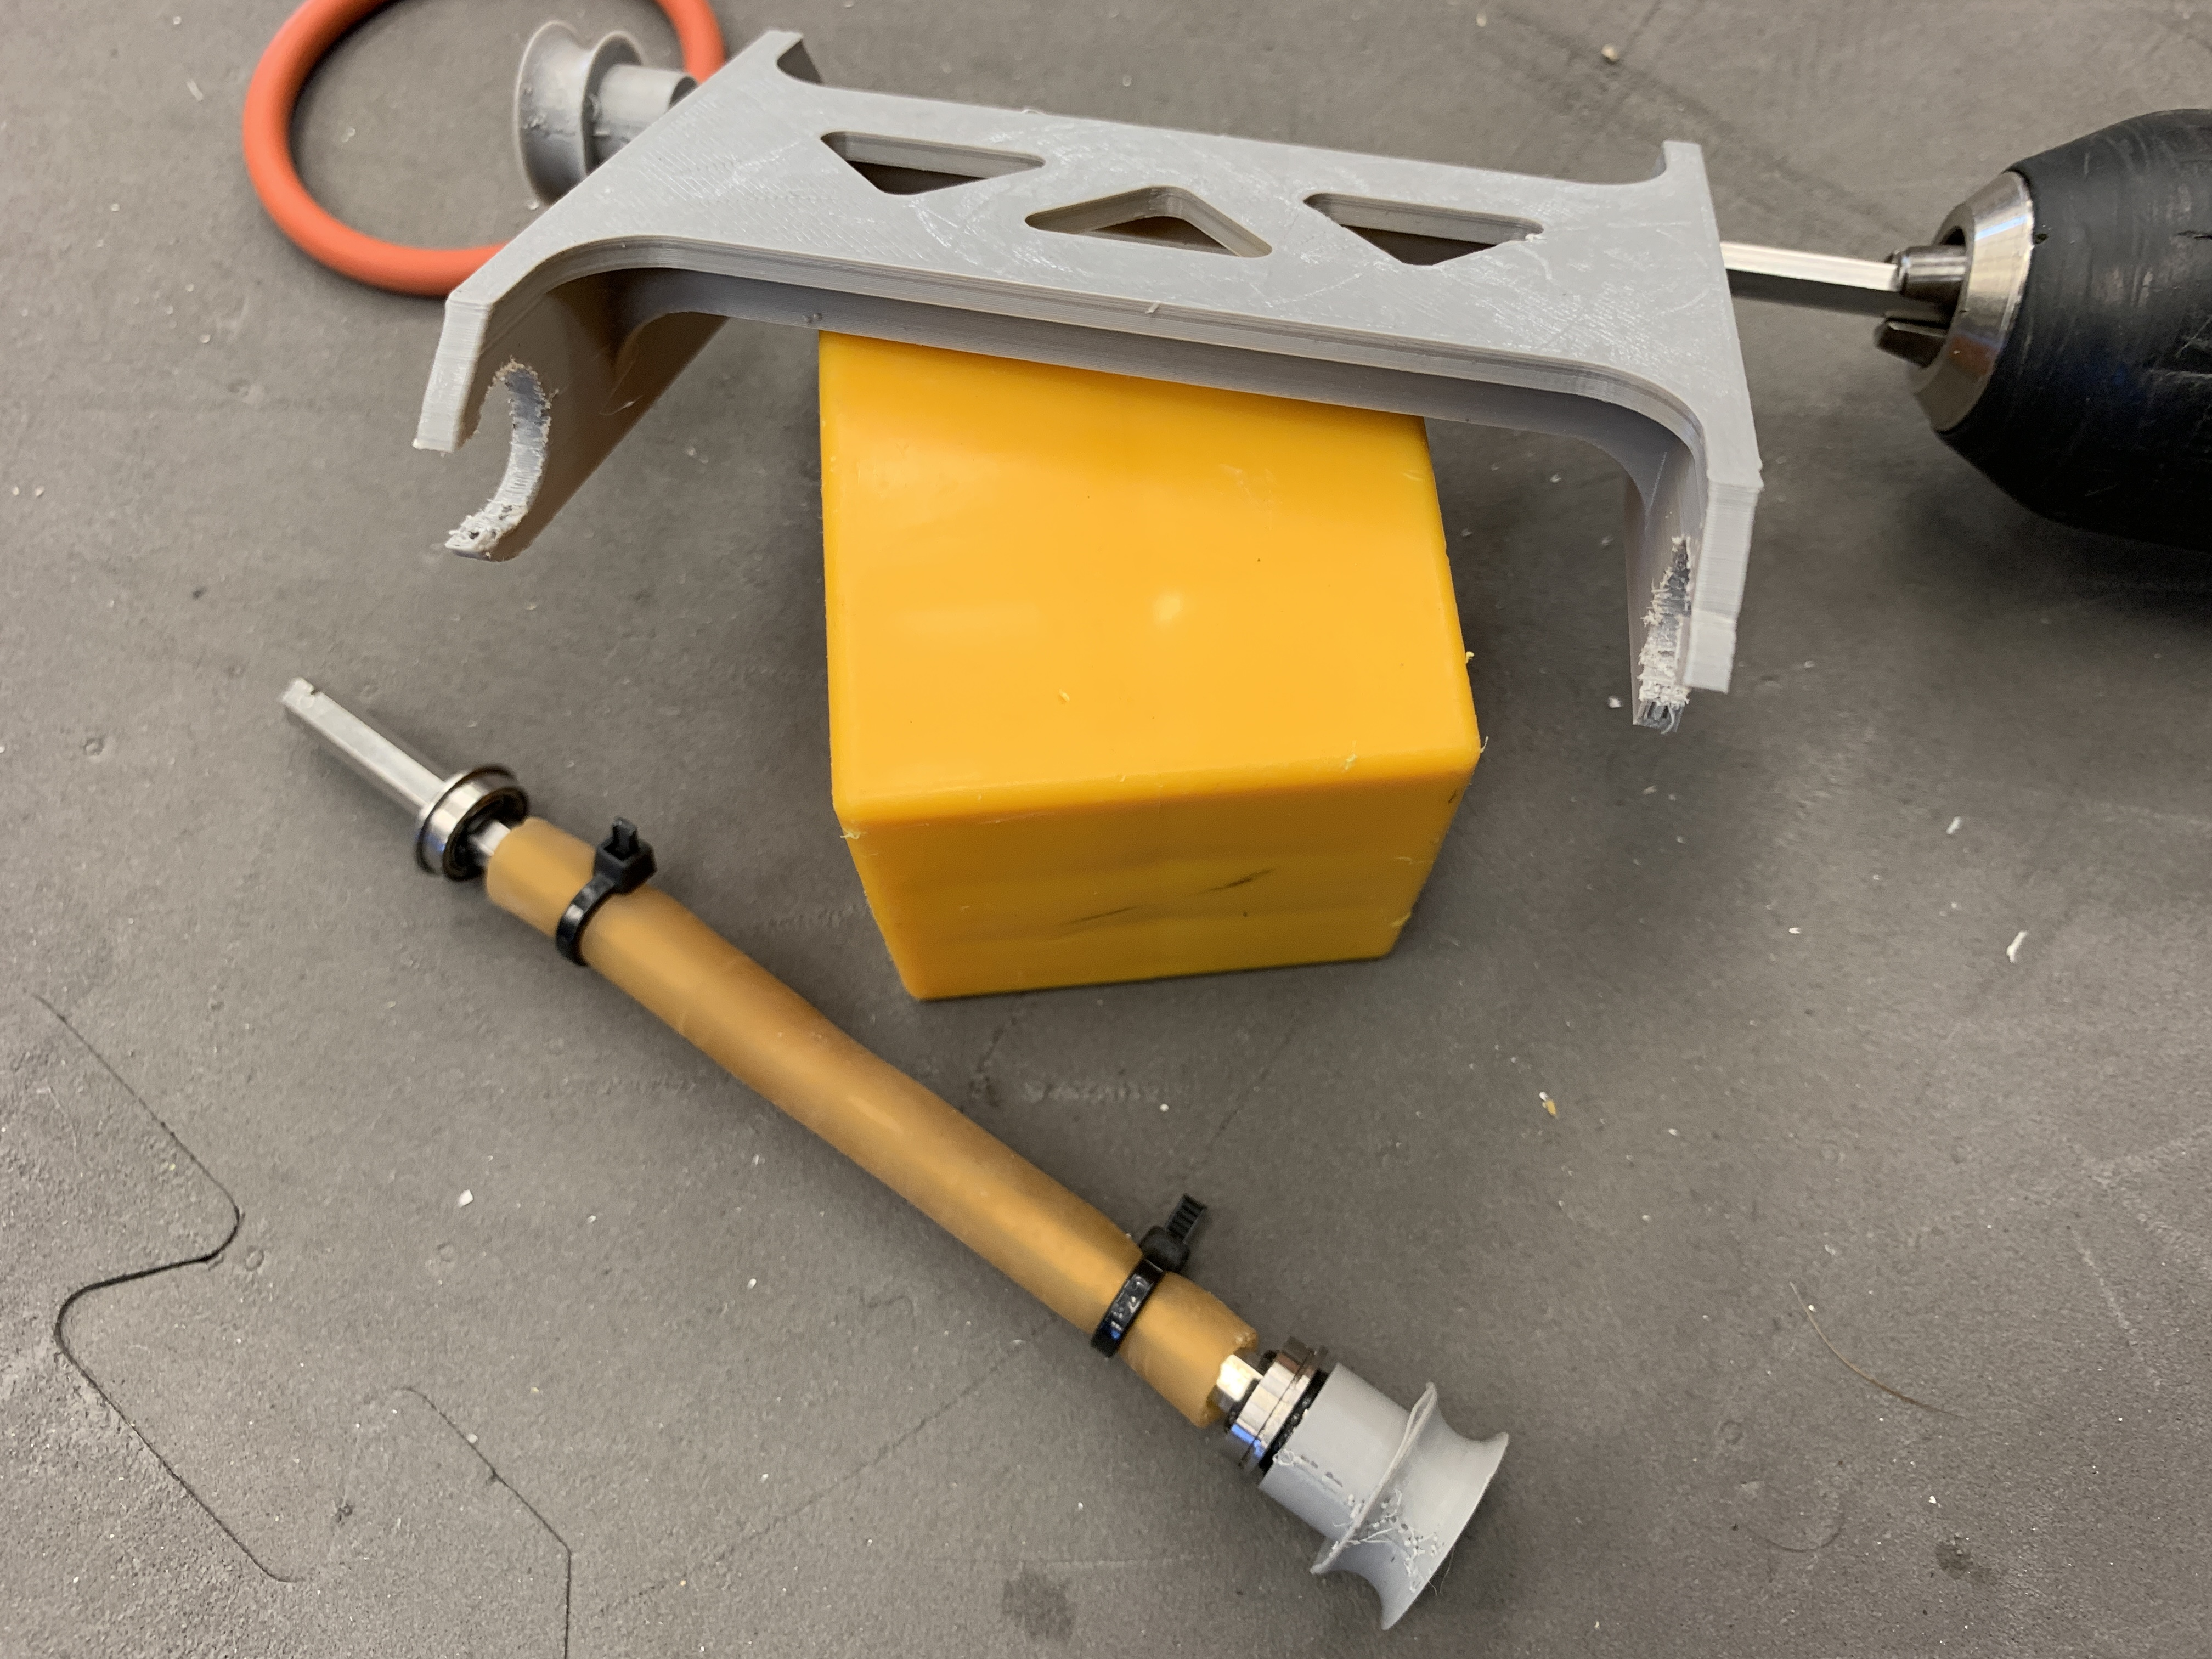
\includegraphics[width=0.95\textwidth, angle=0]{Meetings/December/12-01-21/12-1-21_Hardware_Figure1 - Nathan Forrer.jpg}
\caption{The spot where the intake cracked}
\label{fig:120121-1}
\end{figure}

\whatsnext{
\begin{itemize}
    \item Continue to work on the new vision and print new circles with a difference in centers
    \item Prepare for upcoming meet
	\item Improve grabber intake to be more reliable and hold onto blocks tighter
	\item Design new side plates
\end{itemize} 
}

